
\section{Introduction}
\label{sec-1}

A space-time raster dataset is a collection of raster layers indexed
by time, or in other words, a time series of raster maps. The \texttt{raster}
package defines the classes \texttt{RasterStack} and \texttt{RasterBrick} to build
multilayer rasters. The index of the collection can be set with the
function \texttt{setZ} (which is not restricted to time indexes). The
\texttt{rasterVis} packages provide several methods to display space-time
rasters.

\subsection{Data}
\label{sec-1-1}
Throughout this chapter we will work with a multilayer raster of daily
solar radiation estimates from CM SAF (section \ref{sec:CMSAF}) falling in
the region of Galicia (north of Spain) during 2011. These data are
arranged in a \texttt{RasterBrick} with 365 layers using \texttt{brick} and time
indexed with \texttt{setZ}.

\index{Packages!raster@\texttt{raster}}
\index{Packages!zoo@\texttt{zoo}}
\index{Packages!rasterVis@\texttt{rasterVis}}
\index{setZ@\texttt{setZ}}

\lstset{language=R,numbers=none}
\begin{lstlisting}
library(raster)
library(zoo)
library(rasterVis)

SISdm <- brick('data/SISgal')

timeIndex <- seq(as.Date('2011-01-01'), by='day', length=365)
SISdm <- setZ(SISdm, timeIndex)
names(SISdm) <- format(timeIndex, '%a_%Y%m%d')
\end{lstlisting}
\section{Level Plots}
\label{sec-2}

This multilayer raster can be displayed with each snapshot in a
panel using the small-multiple technique. The problem with this
approach is that only a limited number of panels can be correctly
displayed on one page. In this example, we print the first 12
days of the sequence (Figure \ref{fig:SISdm}).

\index{levelplot@\texttt{levelplot}}

\lstset{language=R,numbers=none}
\begin{lstlisting}
levelplot(SISdm, layers=1:12, panel=panel.levelplot.raster)
\end{lstlisting}

\begin{figure}[htb]
\centering
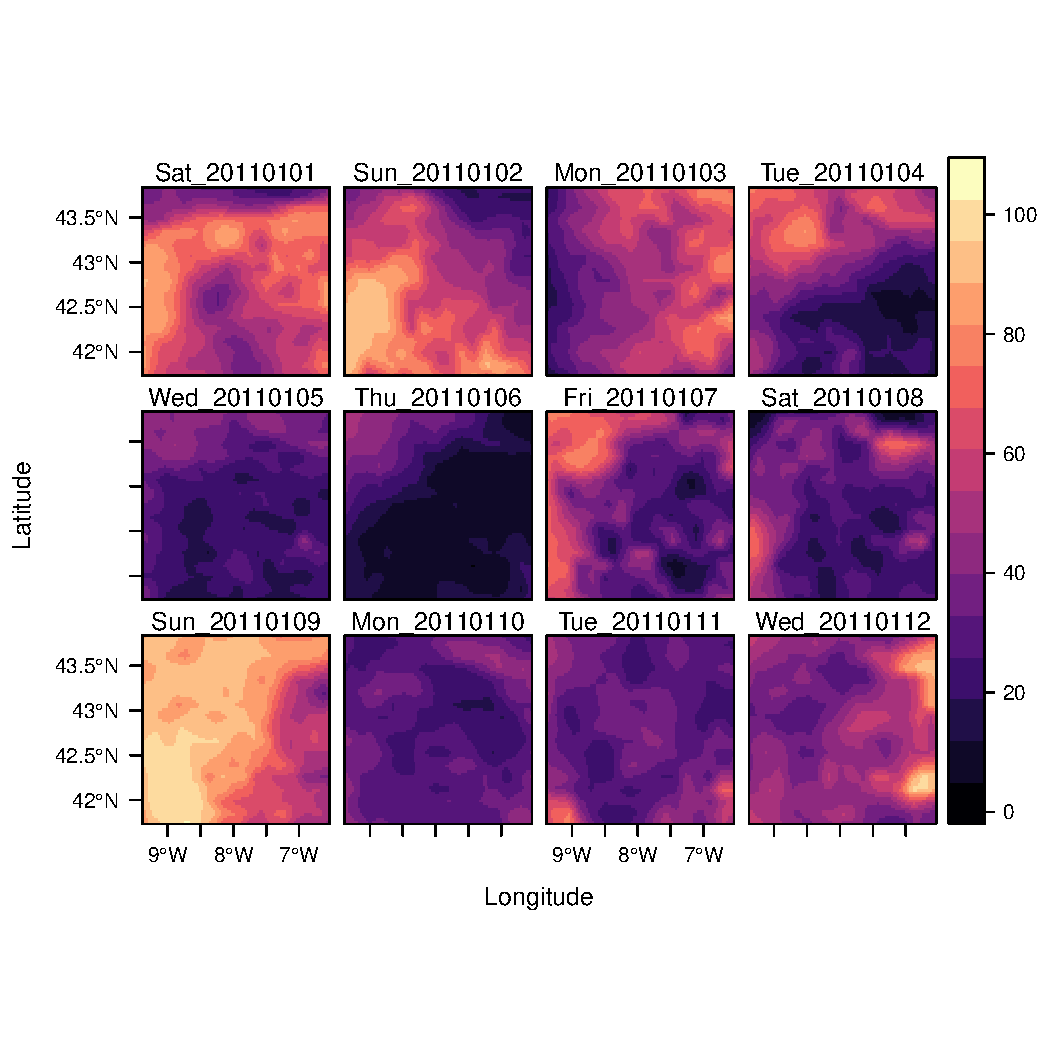
\includegraphics[width=.9\linewidth]{figs/SISdm.pdf}
\caption{\label{fig:SISdm}Level plot of daily averages of solar radiation.}
\end{figure}

When the number of layers is very high, a partial solution is to
aggregate the data, grouping the layers according to a time
condition. For example, we can build a new space-time raster with
the monthly averages using \texttt{zApply} and \texttt{as.yearmon}. This raster
can be completely displayed on one page (Figure \ref{fig:SISmm}),
although part of the information of the original data is lost in
the aggregation procedure.

\index{zApply@\texttt{zApply}}

\lstset{language=R,numbers=none}
\begin{lstlisting}
SISmm <- zApply(SISdm, by=as.yearmon, fun='mean')
\end{lstlisting}

\lstset{language=R,numbers=none}
\begin{lstlisting}
levelplot(SISmm, panel=panel.levelplot.raster)
\end{lstlisting}

\begin{figure}[htb]
\centering
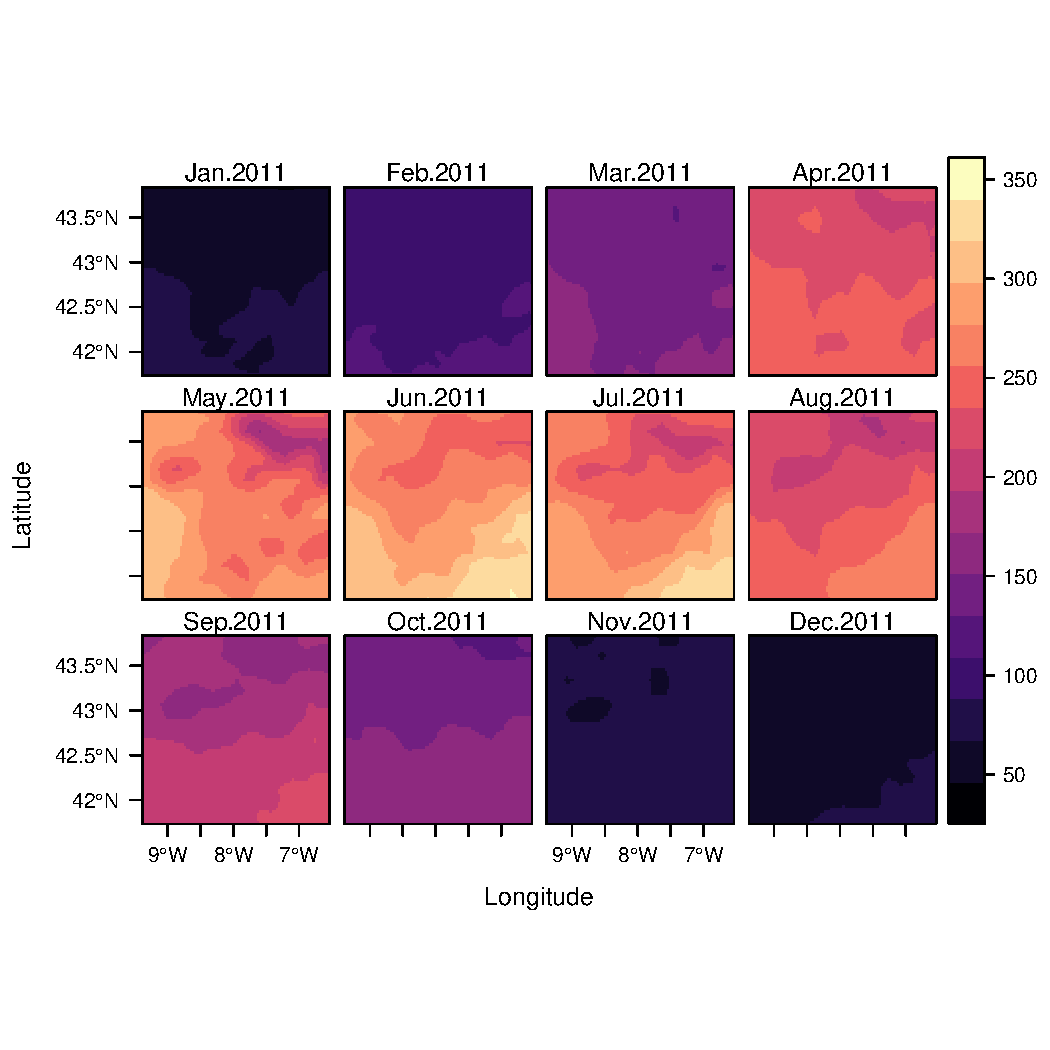
\includegraphics[width=.9\linewidth]{figs/SISmm.pdf}
\caption{\label{fig:SISmm}Level plot of monthly averages of solar radiation.}
\end{figure}
\section{Graphical Exploratory Data Analysis}
\label{sec-3}

There are other graphical tools that complement the previous maps. The
scatterplot and the matrix of scatterplots, the histogram and kernel
density plot, and the boxplot are among the most important tools in
the frame of the Exploratory Data Analysis approach. Some of them were
previously used with a spatial raster (Chapter \ref{cha:raster}). In
this section we will use the histogram (Figure \ref{fig:SISdm_hist}),
the violin plot (a combination of a boxplot and a kernel density plot)
(Figure \ref{fig:SISdm_boxplot}), and the matrix of scatterplots
(section \ref{SEC:groupVariable}, Figure \ref{fig:SISmm_splom}).

\index{histogram@\texttt{histogram}}

\lstset{language=R,numbers=none}
\begin{lstlisting}
histogram(SISdm, FUN=as.yearmon)
\end{lstlisting}

\begin{figure}[htb]
\centering
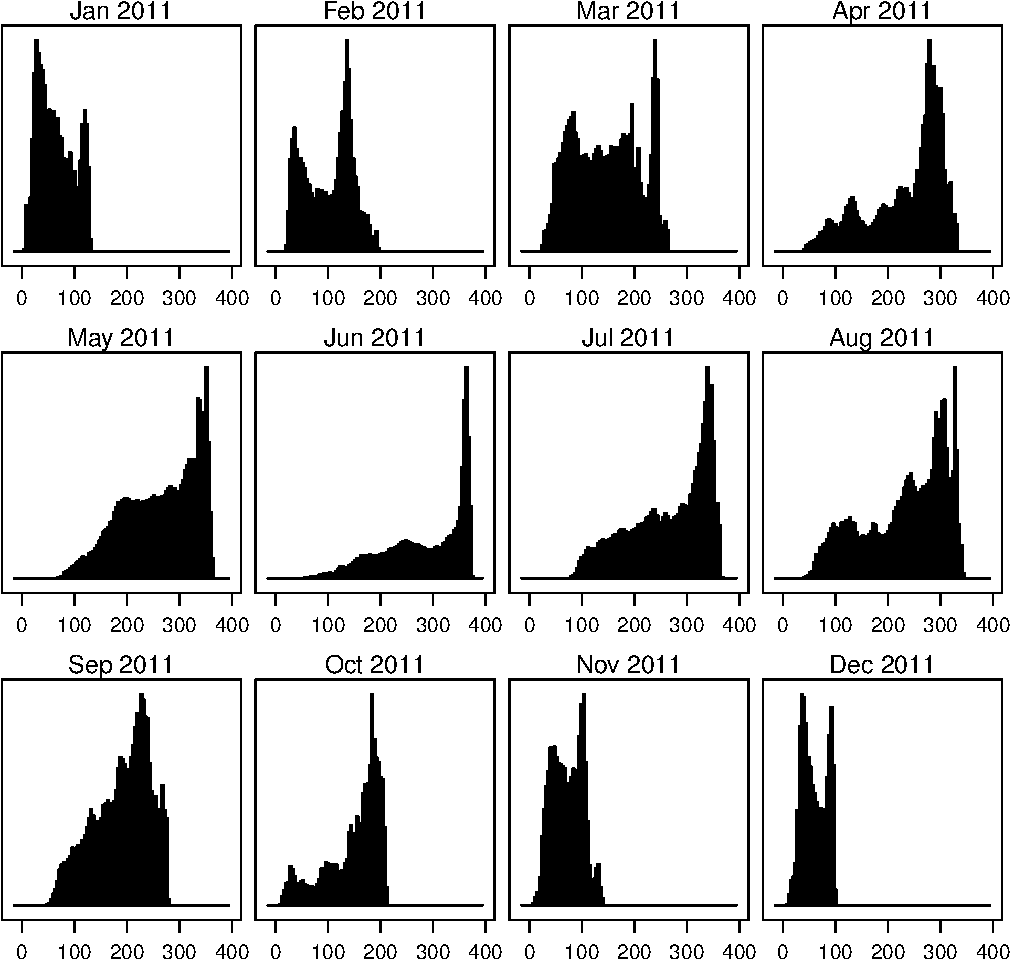
\includegraphics[width=.9\linewidth]{figs/SISdm_histogram.pdf}
\caption{\label{fig:SISdm_hist}Histogram of monthly distribution of solar radiation.}
\end{figure}


\index{bwplot@\texttt{bwplot}}
\lstset{language=R,numbers=none}
\begin{lstlisting}
bwplot(SISdm, FUN=as.yearmon)
\end{lstlisting}

\begin{figure}[htb]
\centering
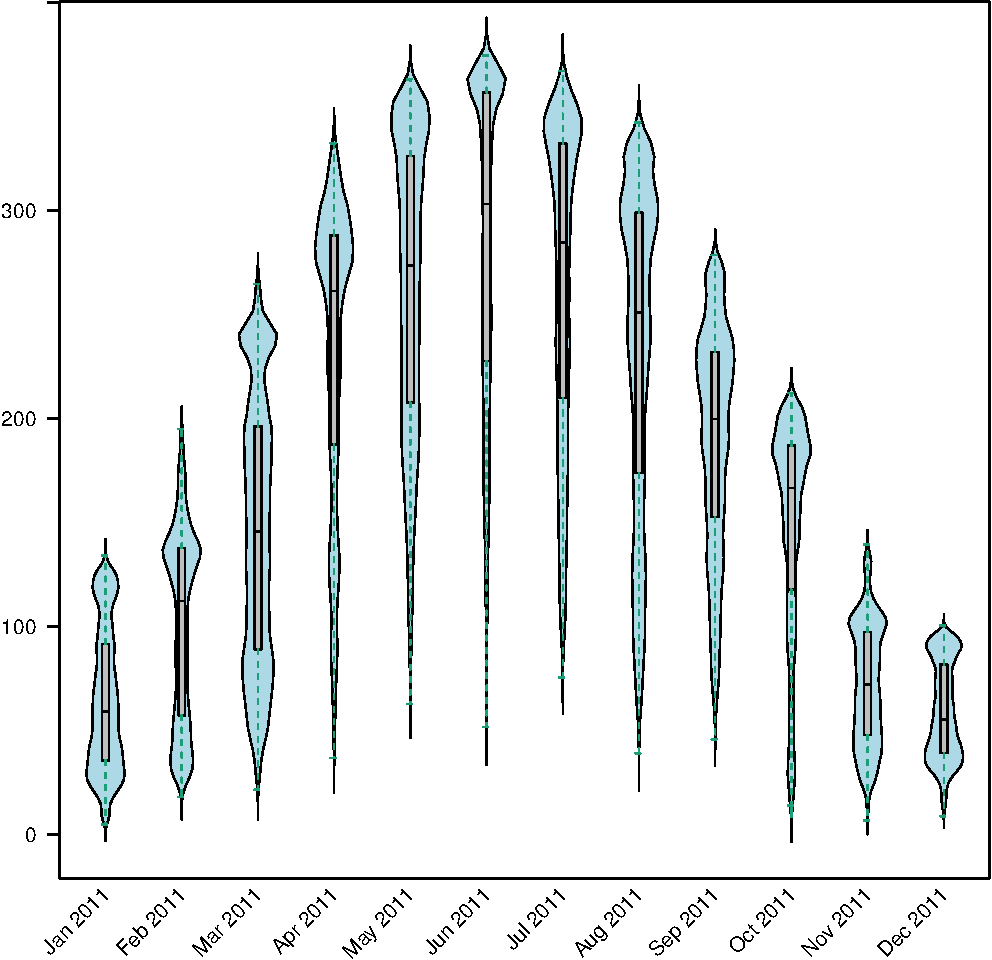
\includegraphics[width=.9\linewidth]{figs/SISdm_boxplot.pdf}
\caption{\label{fig:SISdm_boxplot}Violin plot of monthly distribution of solar radiation.}
\end{figure}

\index{splom@\texttt{splom}}

\lstset{language=R,numbers=none}
\begin{lstlisting}
splom(SISmm, xlab='', plot.loess=TRUE)
\end{lstlisting}

\begin{figure}[htb]
\centering
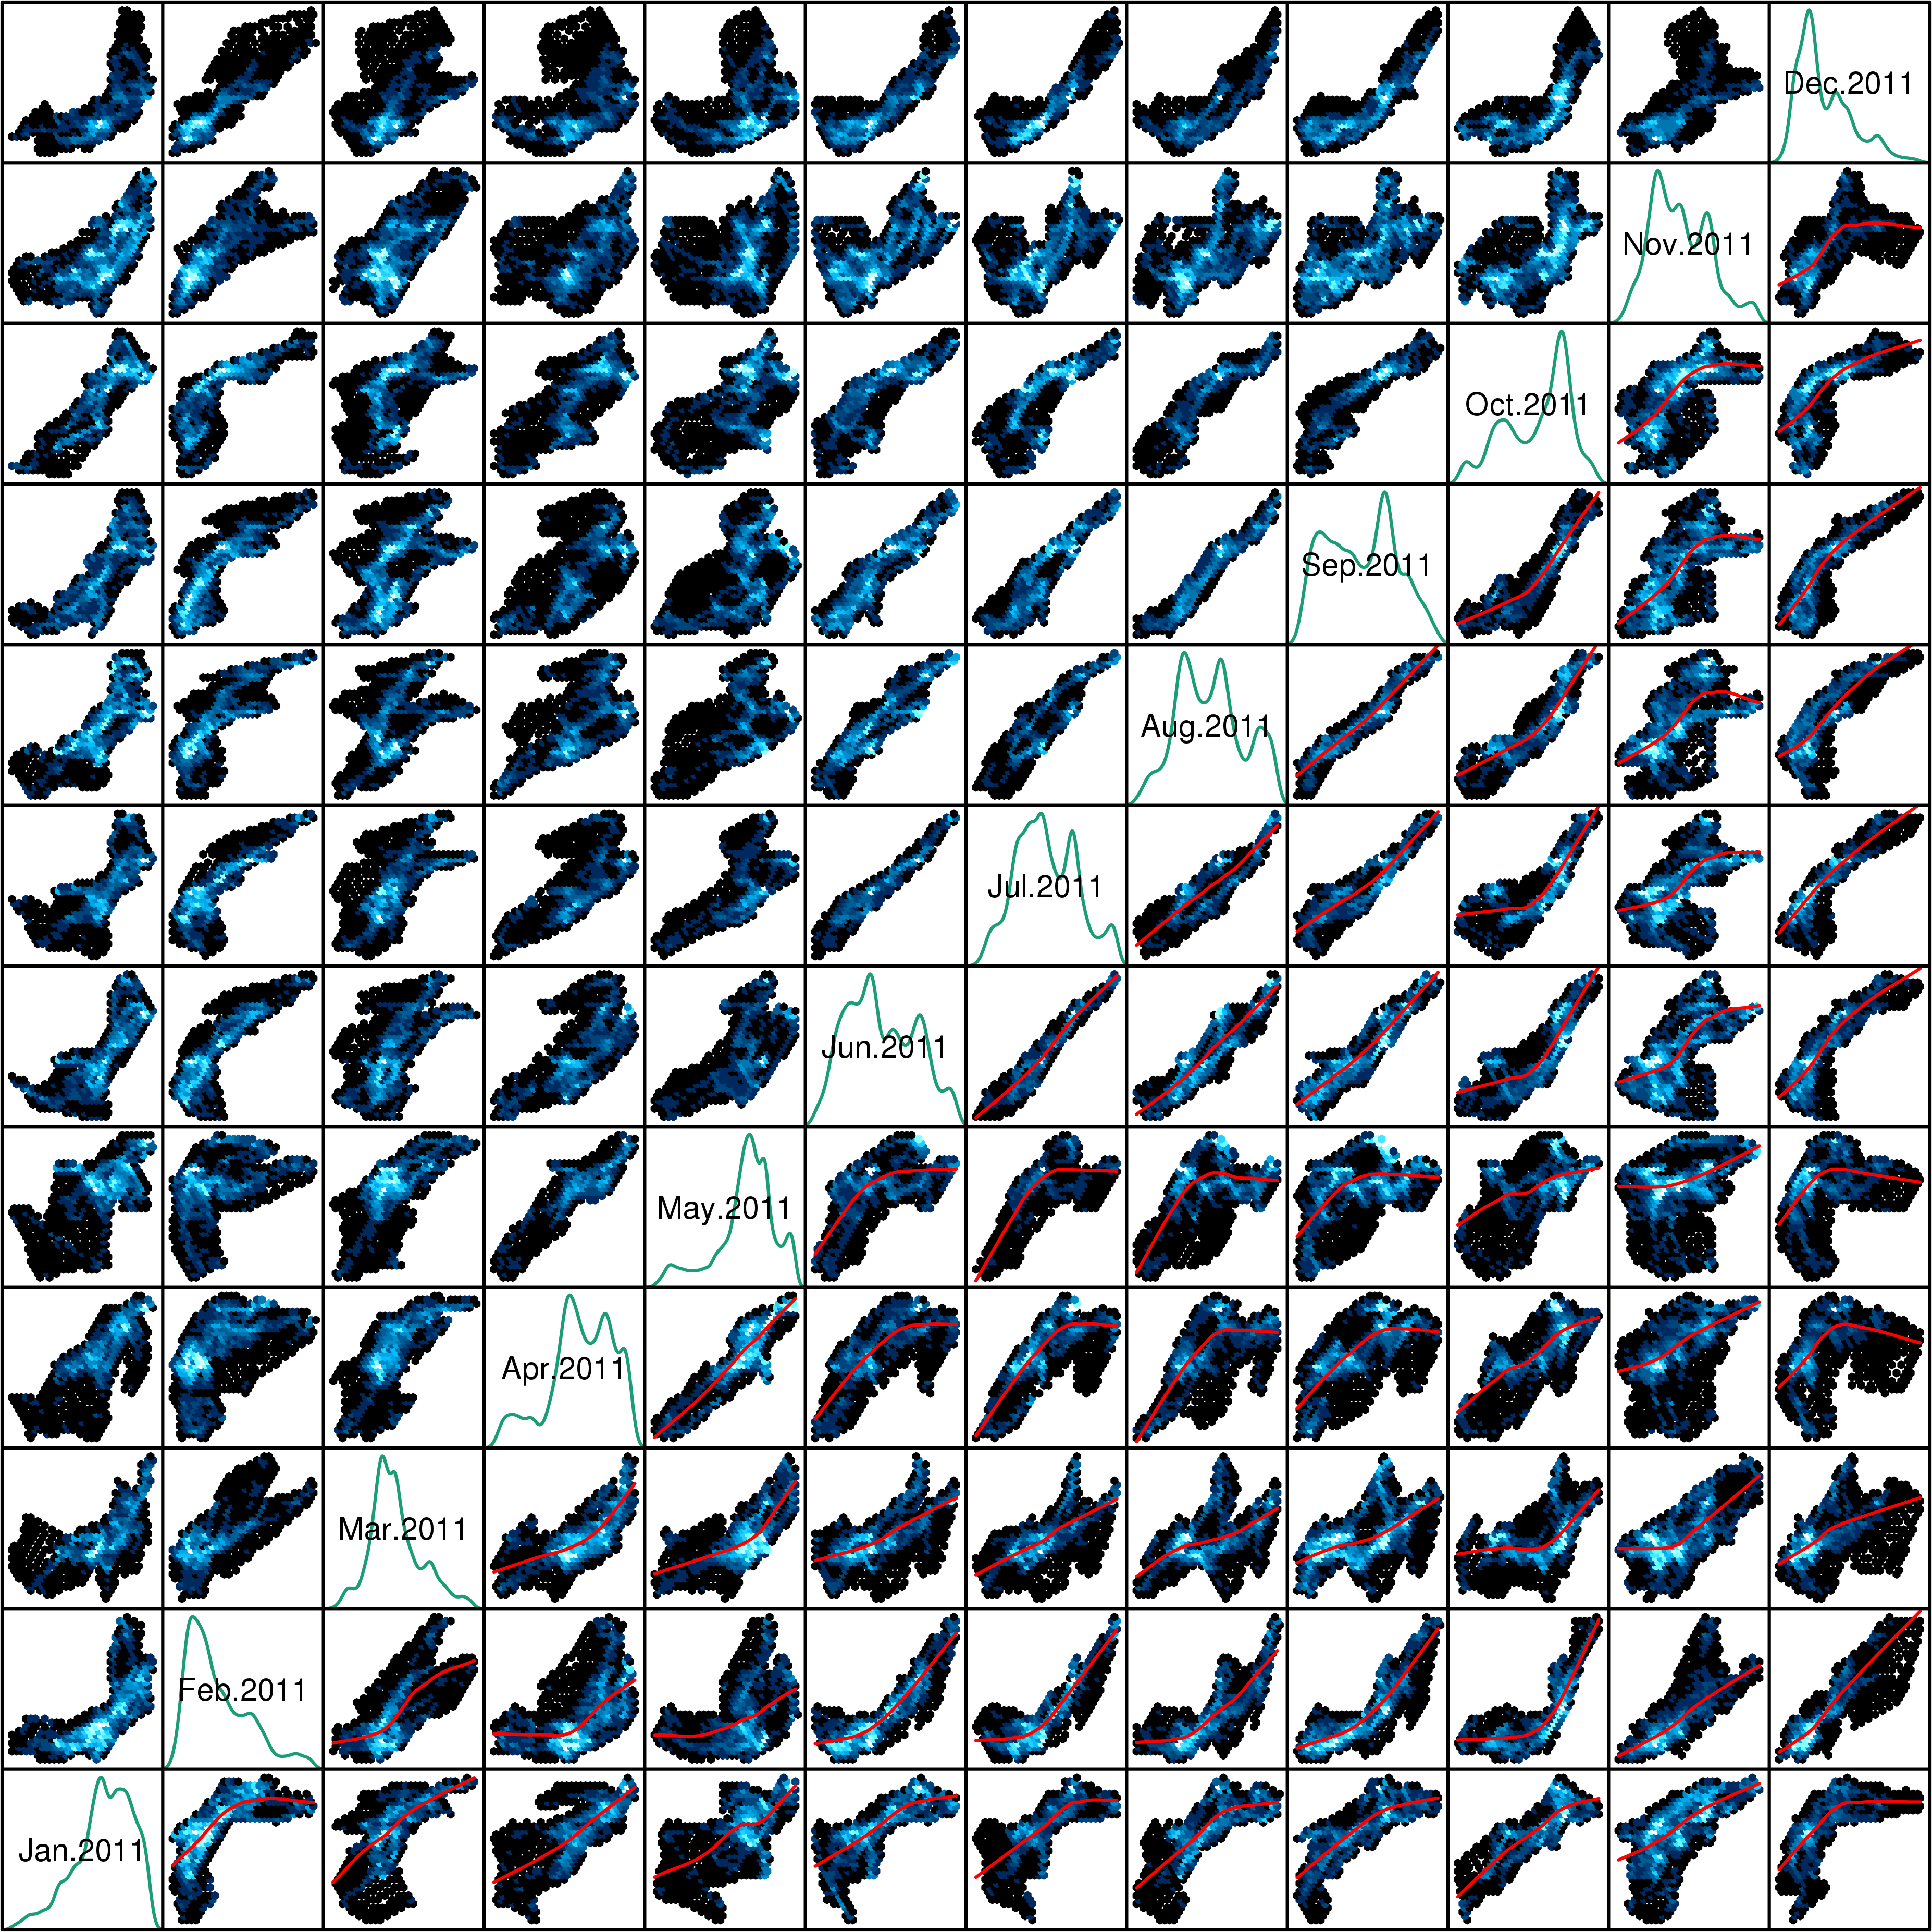
\includegraphics[width=.9\linewidth]{figs/SISmm_splom.png}
\caption{\label{fig:SISmm_splom}Scatterplot matrix of monthly averages together with their kernel density estimations in the diagonal frames.}
\end{figure}


Both the histogram and the violin plot show that daily solar
irradiation is bimodal almost every month. This is related to the
predominance of clear sky and overcast days, with several partly
cloudy days between these modes. This geographical region receives
higher irradiation levels from June to September, and both the levels
and the shape of the probability distribution contrast sharply with
the winter.

The matrix of scatterplots displays a quasilinear relationship
between the central months due to the predominance of clear sky
conditions. However, the relationships involving winter months become
strongly nonlinear due to the presence of clouds.
\section{Space-Time and Time Series Plots}
\label{sec-4}
The level plots of Figures \ref{fig:SISdm} and \ref{fig:SISmm}
display the full 3D space-time with a grid of panels where each layer
is printed. In other words, the raster is sliced, and the collection of
pieces is shown in a table. In the section \ref{sec:animationST}, this
collection of layers will be displayed sequentially like frames of a
movie to build an animation. In this section, the 3D raster is reduced
to a 2D matrix with spatial aggregation following a certain
direction. For example, Figure \ref{fig:SISdm_hovmoller_lat}
displays with colors the averaged value of the raster for each
latitude zone (using the default value of the argument \texttt{dirXY}) with
time on the vertical axis.

\index{hovmoller@\texttt{hovmoller}}

\lstset{language=R,numbers=none}
\begin{lstlisting}
hovmoller(SISdm, par.settings=BTCTheme())
\end{lstlisting}

\begin{figure}[htb]
\centering
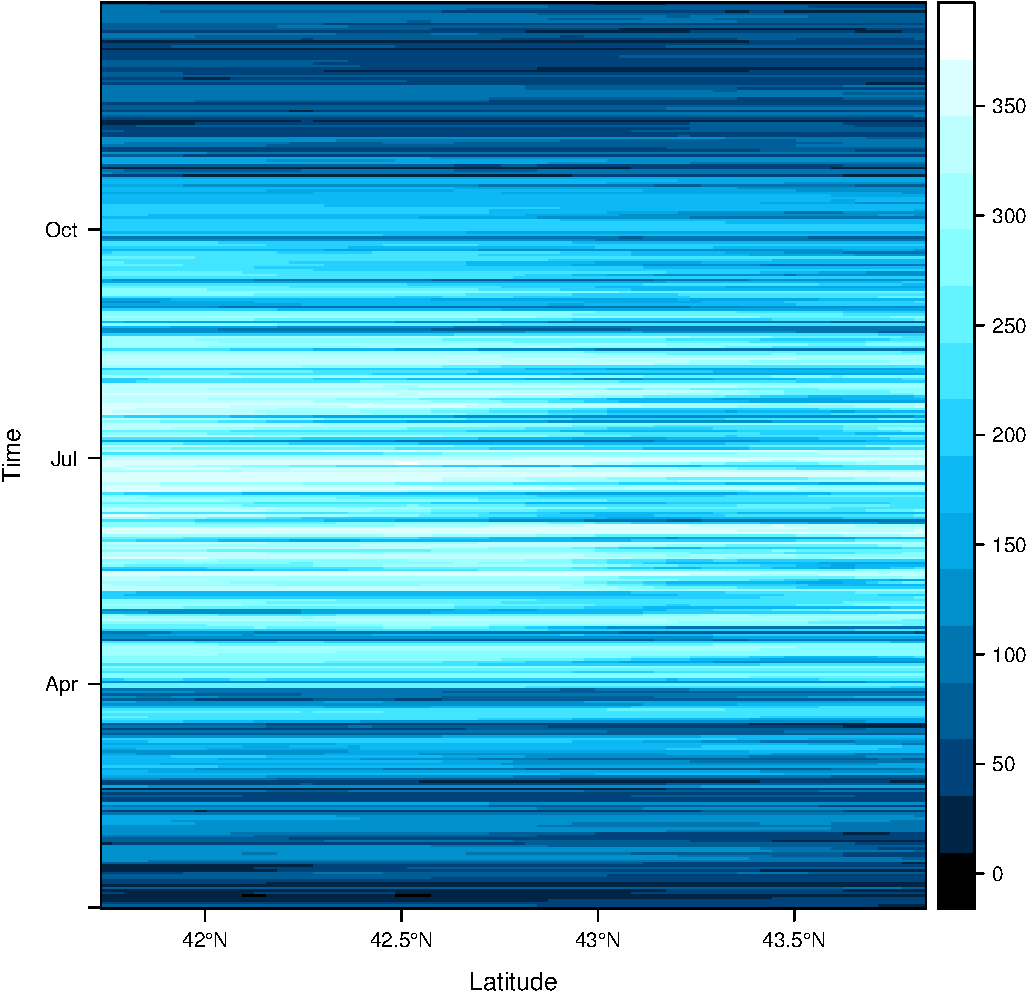
\includegraphics[width=.9\linewidth]{figs/SISdm_hovmoller_lat.pdf}
\caption{\label{fig:SISdm_hovmoller_lat}Hovmöller graphic displaying the time evolution of the average solar radiation for each latitude zone.}
\end{figure}

On the other hand, this 2D matrix can be conceived as a multivariate
time series with each aggregated zone conforming to a different variable of
the time series. This approach is followed by the \texttt{xyplot} (Figure
\ref{fig:SISmm_xyplot}) and \texttt{horizonplot} (Figure \ref{fig:SISdm_horizonplot})
methods, which reproduce the procedures described in Chapter
\ref{cha:timeHorizontalAxis} to display multivariate time series.

\index{xyplot@\texttt{xyplot}}

\lstset{language=R,numbers=none}
\begin{lstlisting}
xyplot(SISdm, digits=1, col='black', lwd=0.2, alpha=0.6)
\end{lstlisting}

\begin{figure}[htb]
\centering
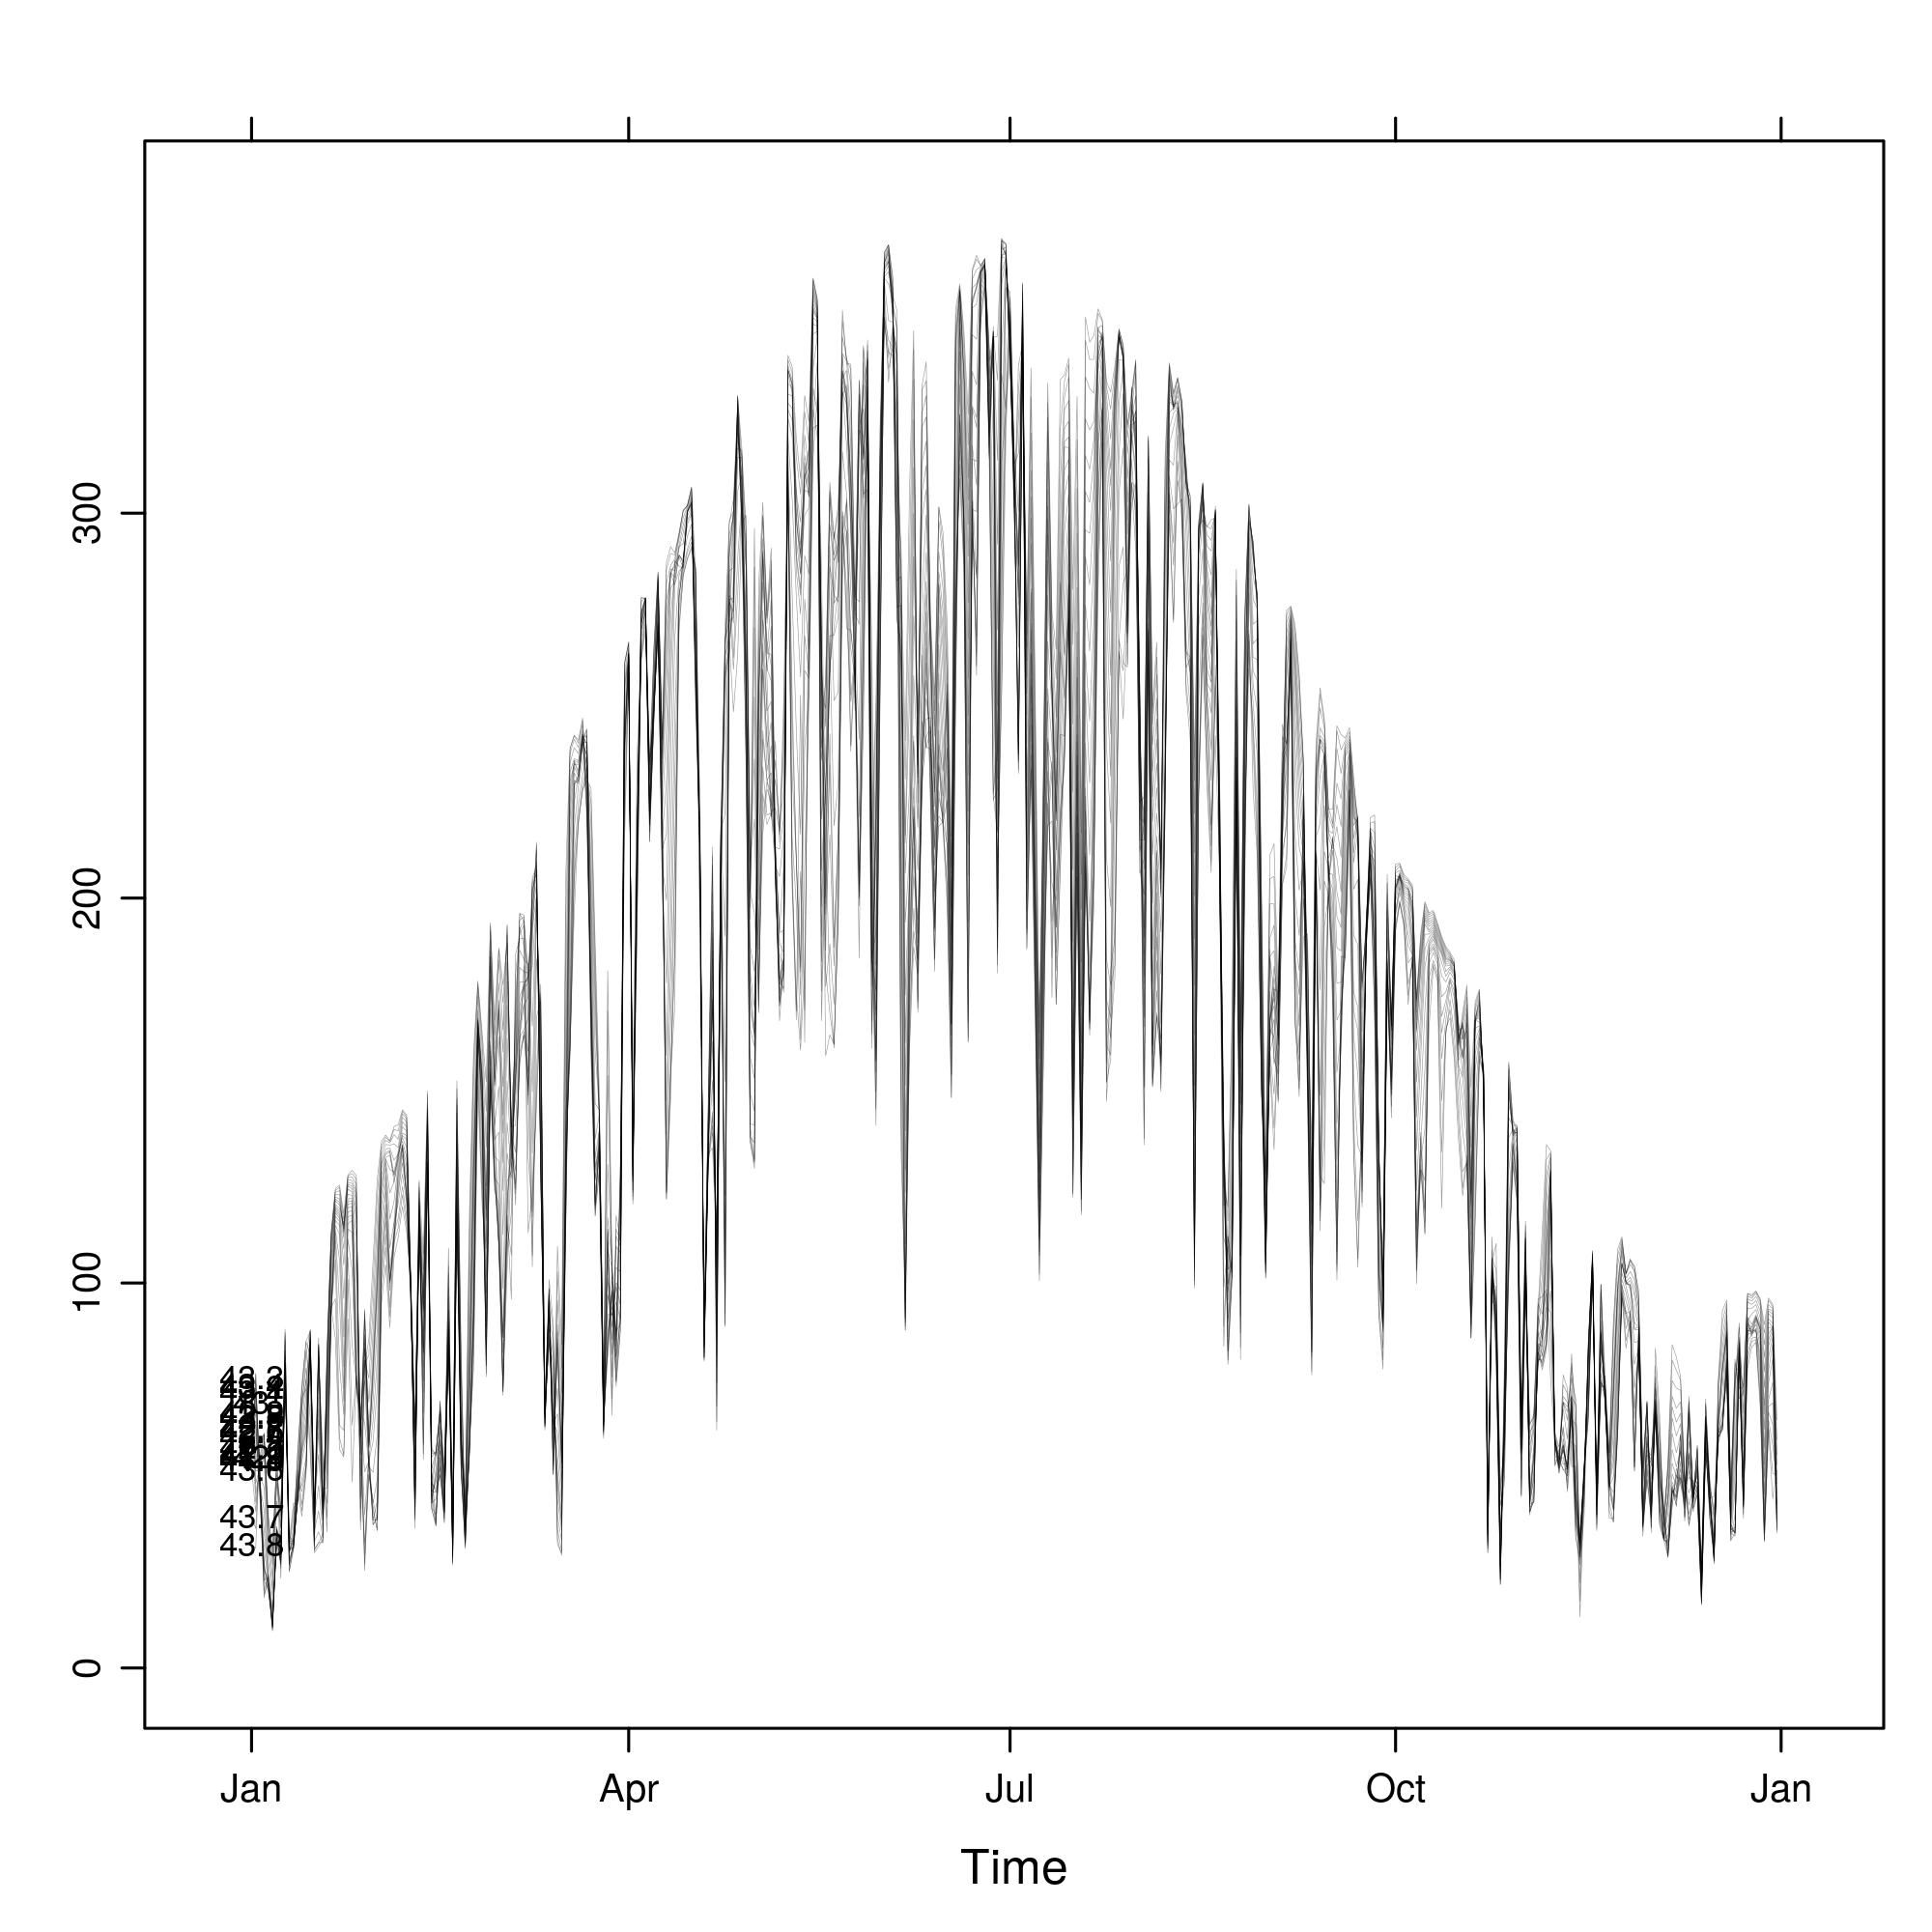
\includegraphics[width=.9\linewidth]{figs/SISmm_xyplot.png}
\caption{\label{fig:SISmm_xyplot}Time graph of the average solar radiation for each latitude zone. Each line represents a latitude band.}
\end{figure}

\index{horizonplot@\texttt{horizonplot}}

\lstset{language=R,numbers=none}
\begin{lstlisting}
horizonplot(SISdm, digits=1,
	    col.regions=rev(brewer.pal(n=6, 'PuOr')),
	    xlab='', ylab='Latitude')
\end{lstlisting}

\begin{figure}[htb]
\centering
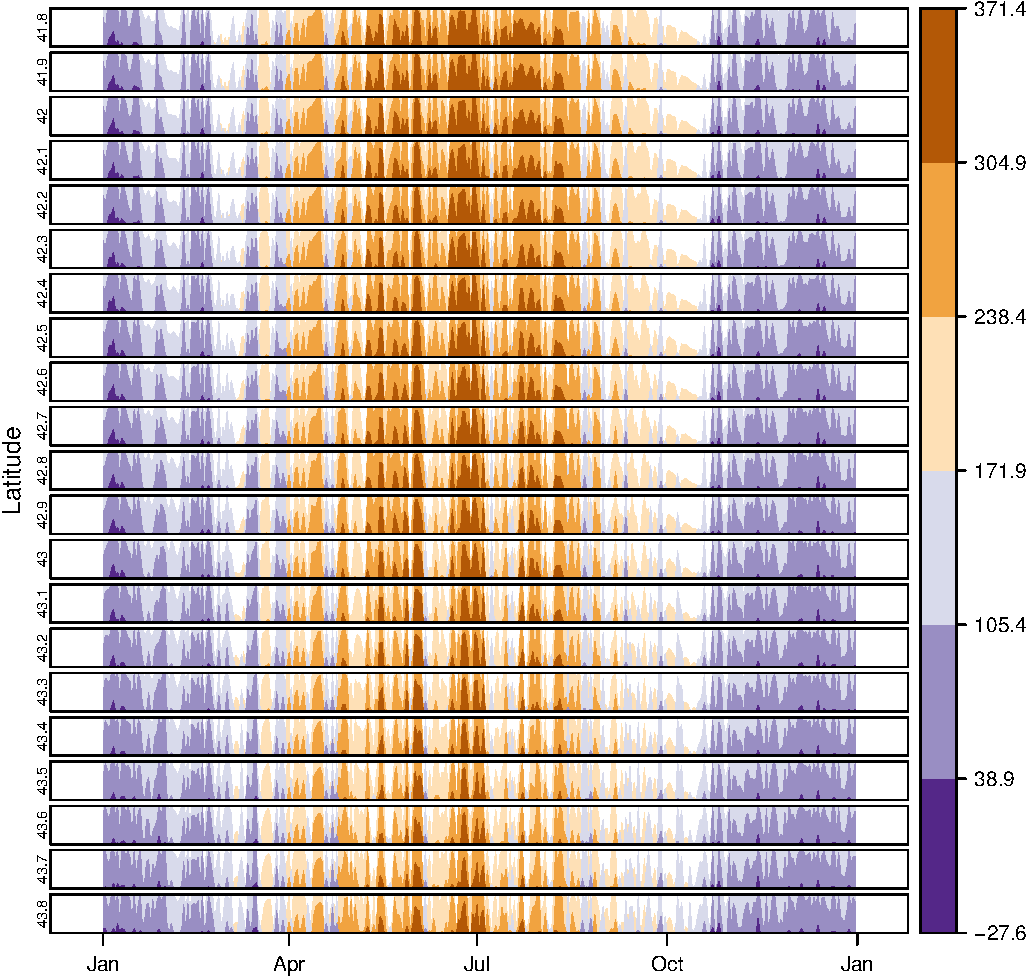
\includegraphics[width=.9\linewidth]{figs/SISdm_horizonplot.pdf}
\caption{\label{fig:SISdm_horizonplot}Horizon graph of the average solar radiation for each latitude zone.}
\end{figure}

These three figures highlight the stational behavior of the solar
radiation, with higher values during the central months. It is
interesting to note that (Figure \ref{fig:SISdm_horizonplot}) the
radiation values around the equinoxes fluctuate near the yearly
average value of each latitude region.
\section{Animation}
\label{sec-5}
\label{sec:animationST}

A different approach is to plot the individual layers of the
space-time raster sequentially as movie frames to produce an
animation. The procedure is quite simple:
\begin{itemize}
\item Plot each layer of the raster to produce a collection of graphic
files.
\item Join these files as a sequence of frames with a suitable tool (for
example, \texttt{ffmpeg}) to create a movie file\footnote{The \texttt{animation} package \cite{Xie2013} defines several functions to wrap \texttt{ffmpeg} and \texttt{convert} from ImageMagick.}\textsuperscript{,}\,\footnote{An alternative method is the \LaTeX{} animate package, which
provides an interface to create portable JavaScript-driven PDF
animations from rasterized image files.}.
\end{itemize}


The effectiveness of this visualization procedure is partly related to
the similitude between consecutive frames. If the frames of the
sequence diverge excessively from one to another, the user will
experience difficulties to perceive any relationship between them. On
the other hand, if the transitions between layers are smooth enough,
the frames will be perceived as conforming to a whole story; and,
moreover, the user will be able to spot both the stable patterns and
the important variations.

\subsection{Data}
\label{sec-5-1}
The daily solar radiation CM-SAF data do not meet the condition of
a smooth transition between layers. The changes between the consecutive
snapshots of daily radiation are too abrupt to be glued one after
another. We will work with a different dataset in this section.

The THREDSS server\footnote{\url{http://mandeo.meteogalicia.es/thredds/catalogos/WRF_2D/catalog.html}} of Meteogalicia\footnote{\url{http://www.meteogalicia.es}} provides access
through different protocols to the output of a Weather Research
and Forecasting (WRF) model, a mesoscale numerical weather
prediction system. Among the set of available variables we will
use the forecast of hourly cloud cover at low and mid levels. This
space-time raster has a time horizon of 96 hours and a spatial
resolution of 12 kilometers.

\lstset{language=R,numbers=none}
\begin{lstlisting}
cft <- brick('data/cft_20130417_0000.nc')
## use memory instead of file
cft[] <- getValues(cft)
## set projection
projLCC2d <- "+proj=lcc +lon_0=-14.1 +lat_0=34.823 +lat_1=43 +lat_2=43 +x_0=536402.3 +y_0=-18558.61 +units=km +ellps=WGS84"
projection(cft) <- projLCC2d
#set time index
timeIndex <- seq(as.POSIXct('2013-04-17 01:00:00', tz='UTC'), length=96, by='hour')
cft <- setZ(cft, timeIndex)
names(cft) <- format(timeIndex, 'D%d_H%H')
\end{lstlisting}

\subsection{Spatial Context: Administrative Boundaries}
\label{sec-5-2}
Let's provide the spatial context with the countries
boundaries, extracted from the \texttt{worldHires} database of the \texttt{maps}
and \texttt{mapdata} packages.

\index{Packages!maptools@\texttt{maptools}}
\index{Packages!mapdata@\texttt{mapdata}}
\index{Packages!maps@\texttt{maps}}
\index{Packages!rgdal@\texttt{rgdal}}
\index{map2SpatialLines@\texttt{map2SpatialLines}}
\index{spTransform@\texttt{spTransform}}

\lstset{language=R,numbers=none}
\begin{lstlisting}
library(maptools)
library(rgdal)
library(maps)
library(mapdata)


projLL <- CRS('+proj=longlat +datum=WGS84 +ellps=WGS84 +towgs84=0,0,0')
cftLL <- projectExtent(cft, projLL)
cftExt <- as.vector(bbox(cftLL))
boundaries <- map('worldHires',
		  xlim=cftExt[c(1,3)], ylim=cftExt[c(2,4)],
		  plot=FALSE)
boundaries <- map2SpatialLines(boundaries, proj4string=projLL)
boundaries <- spTransform(boundaries, CRS(projLCC2d))
\end{lstlisting}

\subsection{Producing the Frames and the Movie}
\label{sec-5-3}
The next step is to produce the collection of frames. We will create a
file with each layer of the \texttt{RasterBrick} using the \texttt{levelplot}
function. This function provides the argument \texttt{layout} to control the
arrangement of a multipanel display. If it is set to \texttt{c(1,1)}, a
different page is created for each layer.

\index{brewer.pal@\texttt{brewer.pal}}
\lstset{language=R,numbers=none}
\begin{lstlisting}
cloudTheme <- rasterTheme(region=brewer.pal(n=9, 'Blues'))
\end{lstlisting}

\index{levelplot@\texttt{levelplot}}

\lstset{language=R,numbers=none}
\begin{lstlisting}
tmp <- tempdir()
trellis.device(png, file=paste0(tmp, '/Rplot%02d.png'),
		      res=300, width=1500, height=1500)
levelplot(cft, layout=c(1, 1), par.settings=cloudTheme) +
    layer(sp.lines(boundaries, lwd=0.6))
dev.off()
\end{lstlisting}

A suitable tool to concatenate these frames and create the movie is
\texttt{ffmpeg}, a free cross-platform software to record, convert, and stream
audio and video\footnote{\url{http://www.ffmpeg.org/}}. The resulting movie is available from the book
website.

\index{ffmpeg@\texttt{ffmpeg}}

\lstset{language=R,numbers=none}
\begin{lstlisting}
old <- setwd(tmp)
## Create a movie with ffmpeg using 6 frames per second a bitrate of 300kbs
movieCMD <- 'ffmpeg -r 6 -b 300k -i Rplot%02d.png output.mp4'
system(movieCMD)
file.remove(dir(pattern='Rplot'))
file.copy('output.mp4', paste0(old, '/figs/cft.mp4'), overwrite=TRUE)
setwd(old)
\end{lstlisting}
\subsection{Static Image}
\label{sec-5-4}
Figure \ref{fig:cft} shows a sequence of twenty-four snapshots (second day
of the forecast series) of the movie. This graphic is also created
with \texttt{levelplot} but now using the argument \texttt{layers} to choose a
subset of the layers, and with a different value for \texttt{layout} to
display a matrix of twenty-four panels.
\lstset{language=R,numbers=none}
\begin{lstlisting}
levelplot(cft, layers=25:48, layout=c(6, 4),
	  par.settings=cloudTheme,
	  names.attr=paste0(sprintf('%02d', 1:24), 'h'),
	  panel=panel.levelplot.raster) +
    layer(sp.lines(boundaries, lwd=0.6))
\end{lstlisting}

\begin{figure}[htb]
\centering
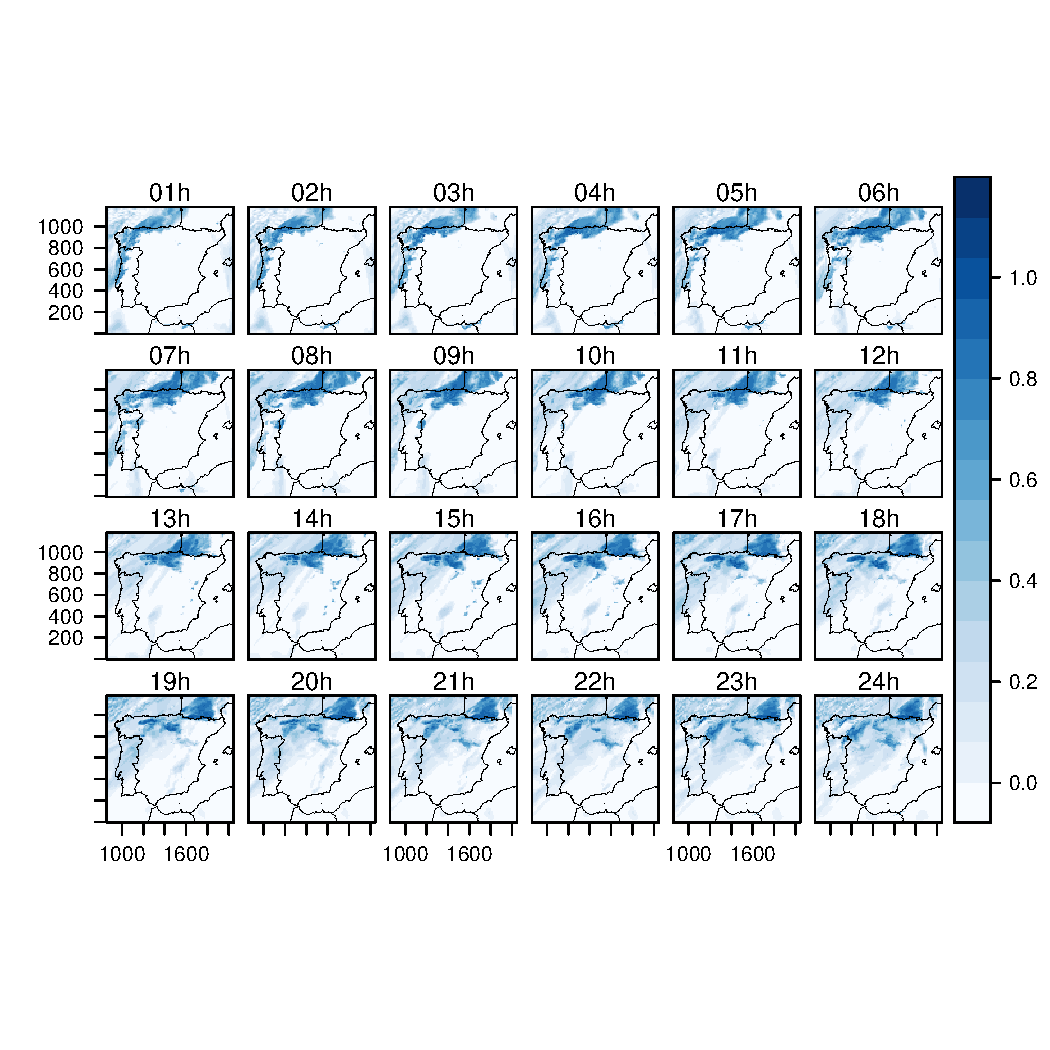
\includegraphics[width=.9\linewidth]{figs/cft.pdf}
\caption{\label{fig:cft}Forecast of hourly cloud cover at low and mid levels.}
\end{figure}

The movie and the static image are complementary tools and should be
used together. Watching the movie you will perceive the cloud transit
from Galicia to the Pyrenees gradually dissolving over the Cantabrian
region. On the other hand, with Figure \ref{fig:cft} you can locate the
position of a group of clouds in a certain hour and simultaneously
observe the relationship of that position with the evolution during
that period. With the movie you will concentrate your attention on the
movement. With small multiple pictures, your focus will be on
positions and relations. You should use both graphical tools to grasp
the entire 3D dataset.
